
\section*{Problem  Set 4}

\subsection*{1.7 Group Actions}


\begin{mdframed}
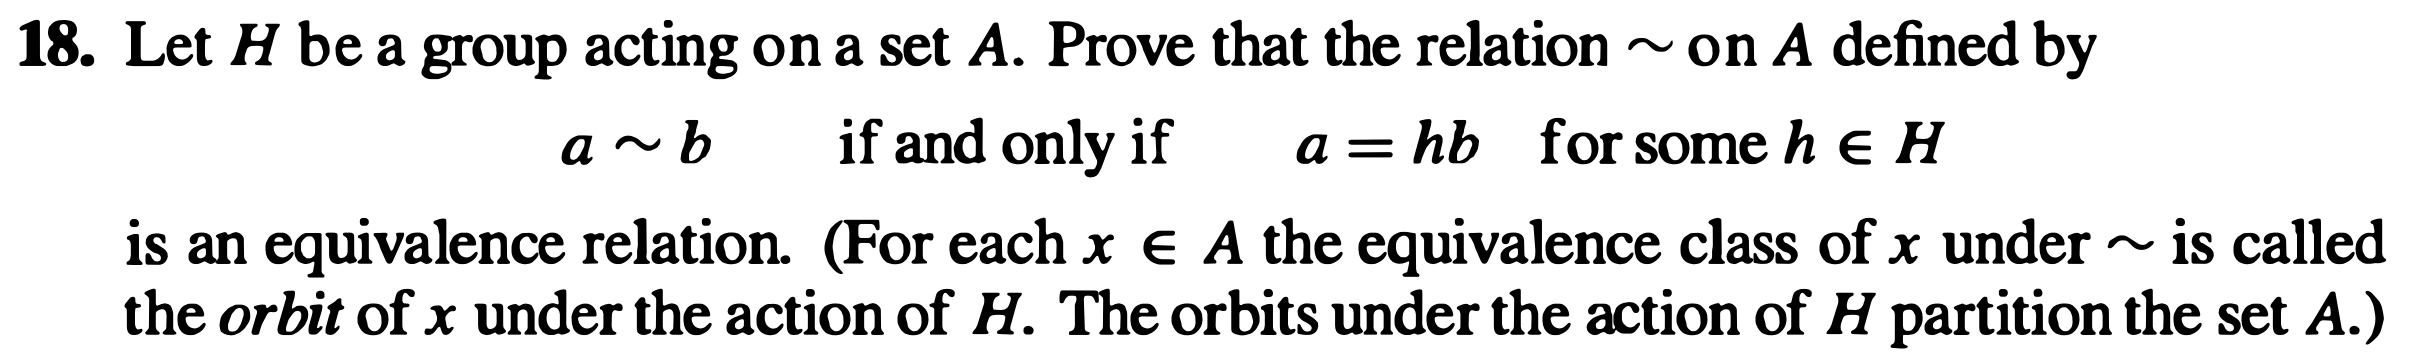
\includegraphics[width=400pt]{img/abstract-algebra--nf--4-bc71.png}
\end{mdframed}

\begin{intuition*}
  Think of the elements of $A$ as vertices of a graph. There's an edge from $a_1$ to $a_2$ if some
  element of $h$ sends $a_1 \mapsto a_2$. Every multi-edge path has a corresponding single edge that goes
  to the same destination. To see that, imagine some path that involves multiple edges; but then
  there's also a single edge connecting the start and end point, given by the composition of the
  multiple edges (group closure means the composition is some other element in the group). It's
  reflexive because every group has an identity. It's symmetric because $h^{-1}$ is the same edge
  as $h$ but with the opposite direction. It's transitive because as we said above, there's always
  a single edge that gets you to the same destination as any two-edge path.
\end{intuition*}

\begin{proof}
  First note that $h$ acts on $A$ as a permutation, and $h^{-1}$ acts on $A$ as the the inverse of
  that permutation. Also note that the identity element acts as the identity permutation because
  the mapping from group elements to the permutations that they act as is a homomorphism, and a
  homomorphism always sends identity to identity.

  {\bf reflexive}\\
  $a \sim a$ since $a = 1a$.

  {\bf symmetric}\\
  If $a \sim b$ then $a = hb$ for some $h \in H$. Therefore $b = h^{-1}a$ hence $b \sim a$.

  {\bf transitive}\\
  If $a \sim b$ and $b \sim c$ then $a = h_1b$ and $b = h_2c$ for some $h_1, h_2 \in H$.
  Therefore $a = (h_1h_2)c$ hence $a \sim c$.
\end{proof}

\newpage
\begin{mdframed}
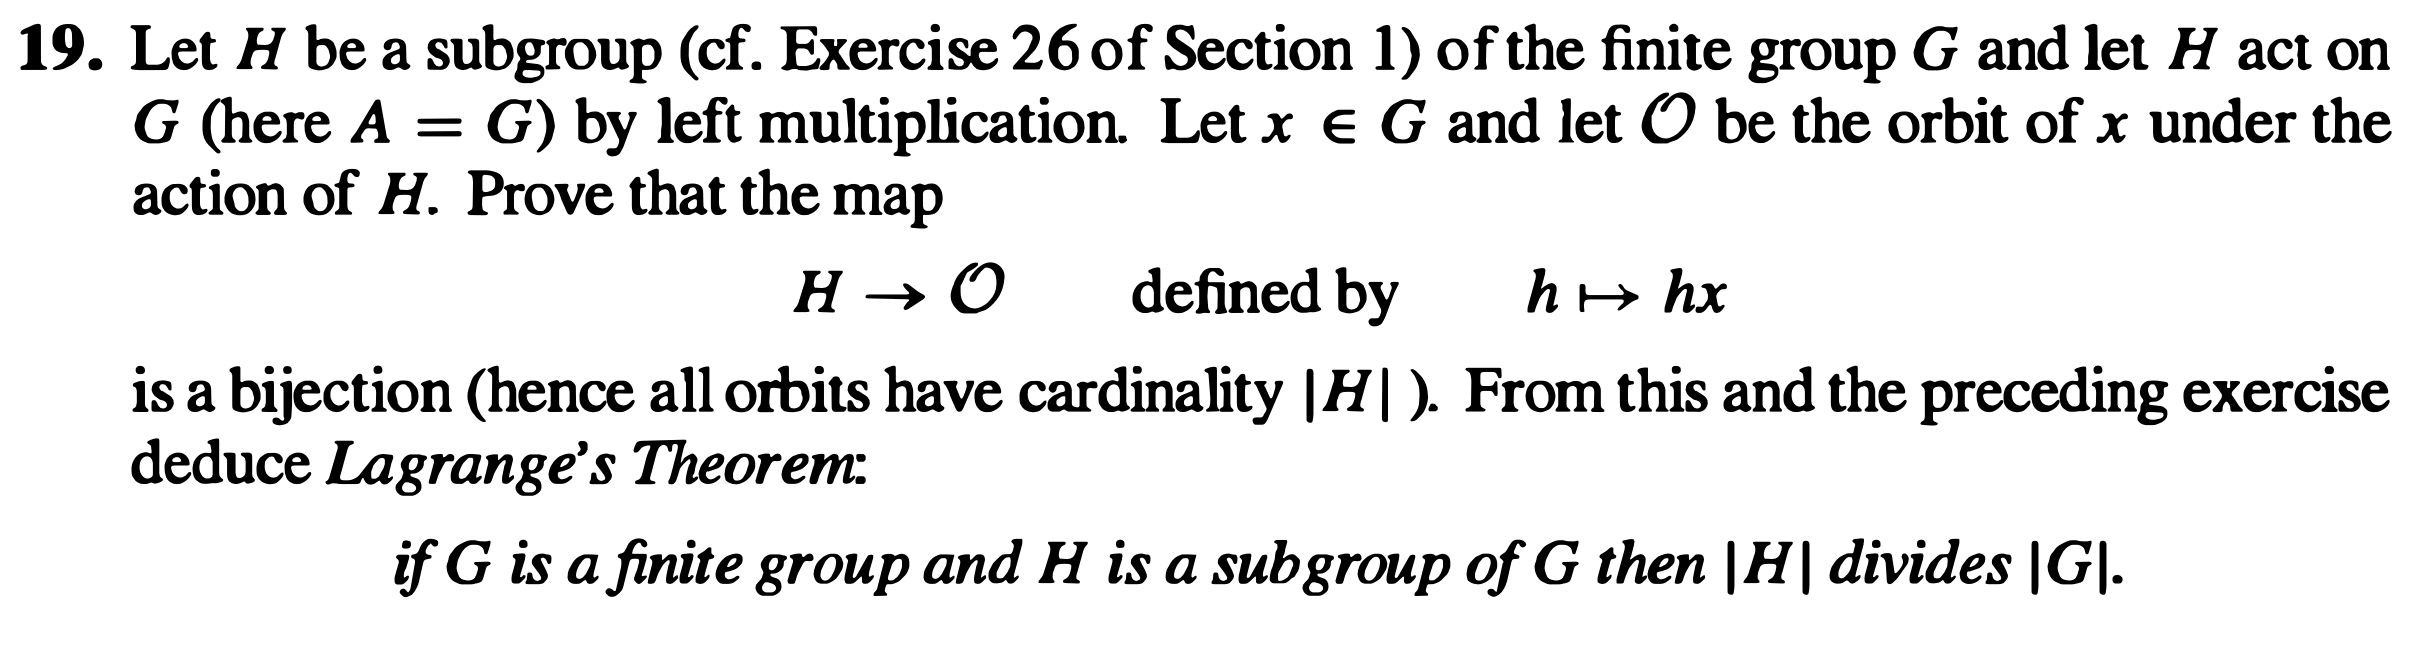
\includegraphics[width=400pt]{img/abstract-algebra--nf--4-4140.png}
\end{mdframed}

\begin{intuition*}
  The map $\varphi$ in question sends $h$ to some element $hx$ of the orbit of $x$ under $H$.
  To get back, right-multiply by $x^{-1}$.
\end{intuition*}

\begin{proof}
  Let $\varphi: H \to \mathcal O$ be the map defined by $h \mapsto hx$.

  The map $\psi: \mathcal O \to H$ defined by $g \mapsto gx^{-1}$ is a left inverse for $\varphi$,
  since $(\psi\varphi)(h) = \psi(\varphi(h)) = (hx)x^{-1} = h$, showing that $\psi\varphi = 1_H$, and also a right inverse
  for $\varphi$, since $(\varphi\psi)(g) = \varphi(\psi(g)) = (gx^{-1})x = g$, showing that $\varphi\psi = 1_G$.

  Therefore $\varphi$ is a bijection, since it has an inverse.

  Therefore the orbit of $x$ under the action of $H$ has cardinality $|H|$ and, since $x$ was
  arbitrary, this is true for the orbit of any $x \in G$ under the action of $H$.

  Since the orbits are equivalence classes, they partition $G$. Therefore $|G| = k|H|$ where $k$ is
  the number of distinct orbits.

  This argument required no assumptions beyond the premise that $H$ is a subgroup of a finite
  group $G$, hence Lagrange's Theorem:

  {\it if $H$ is a subgroup of a finite group $G$, then $H$ divides $|G|$}


  ~\\
.
\end{proof}

\newpage
\begin{mdframed}
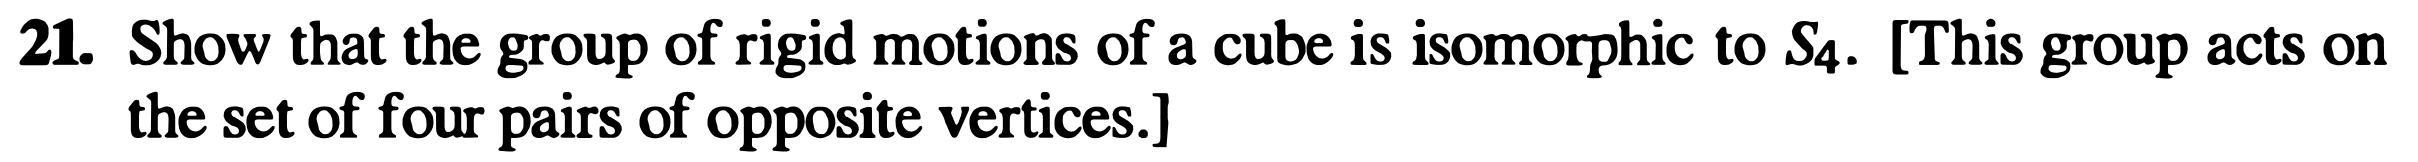
\includegraphics[width=400pt]{img/abstract-algebra--nf--4-0e63.png}
\end{mdframed}

\begin{intuition*}
  Think of $B$ as comprising a red, a blue, a green, and a yellow line, all passing through the
  cube interior, connecting pairs of opposite vertices. If, after a rigid motion of the cube, those
  lines look the same as they did before, then the rigid motion acted on $B$ as the identity
  permutation. (I.e. we do not see any change if the motion of the cube merely reverses the
  orientation of a line; we only see a change if the motion of the cube changes the set of two
  points connected by the line).
\end{intuition*}

\begin{proof}
  Let $B$ be the set of $4$ pairs of opposite vertices of a cube, let $G$ be the group of rigid
  motions of a cube, acting on $B$, and let $\psi: G \to S_B$ be the permutation representation of the
  action of $G$ on $B$.

  We have $|S_B| = 4! = 24$ and also $|G| = 24$. To see this, fix a face of the cube and look at
  the cube face-on; after a rigid motion you are looking at one of the $6$ faces and that face is
  in one of its $4$ rotational configurations, hence $|G| = 6 \times 4 = 24$.

  Next, note that every rigid motion other than the identity acts on $B$ as a non-identity
  permutation. To see this, fix a face of the cube and look at the cube face-on, and label the
  vertices of this ``front​'' face clockwise from top-left as $(b_1, b_2, b_3, b_4)$. Thus if we
  were to look at the opposite ``back​'' face, we'd see the following labels clockwise from
  top-left: $(b_4,b_3,b_2,b_1)$. Now suppose there is a non-identity rigid motion that acts as the
  identity permutation on $B$. Then this rigid motion must move the $b_1$ label at the back to the
  top-left position at the front. But this would move the $b_2$ label at the back to the
  bottom-left position at the front, and so it does not act on $B$ as the identity, since $b_2$
  started off in the top-right position.

  Therefore $\ker \psi = \{1\}$, hence $\psi$ is injective, and also an isomorphism since
  $|G| = |S_B|$, and since $S_B \cong S_4$ and isomorphism is a transitive relation, we have the
  desired result.
\end{proof}



\begin{mdframed}
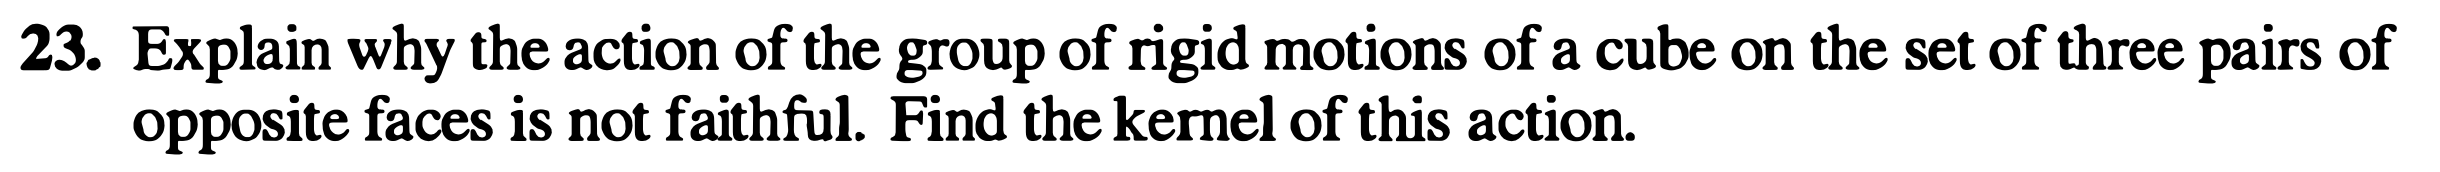
\includegraphics[width=400pt]{img/abstract-algebra--nf--4-5a92.png}
\end{mdframed}

\begin{proof}
  It can't be faithful because there are 24 rigid motions of a cube and 6 permutations of 3 items.
\end{proof}


\begin{mdframed}
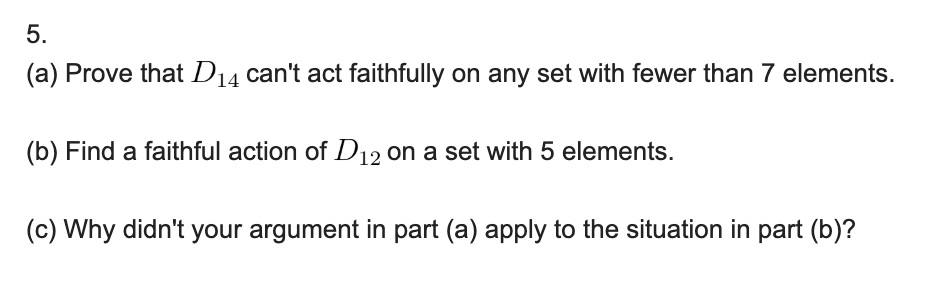
\includegraphics[width=400pt]{img/abstract-algebra--nf--4-1b73.png}
\end{mdframed}





\begin{mdframed}
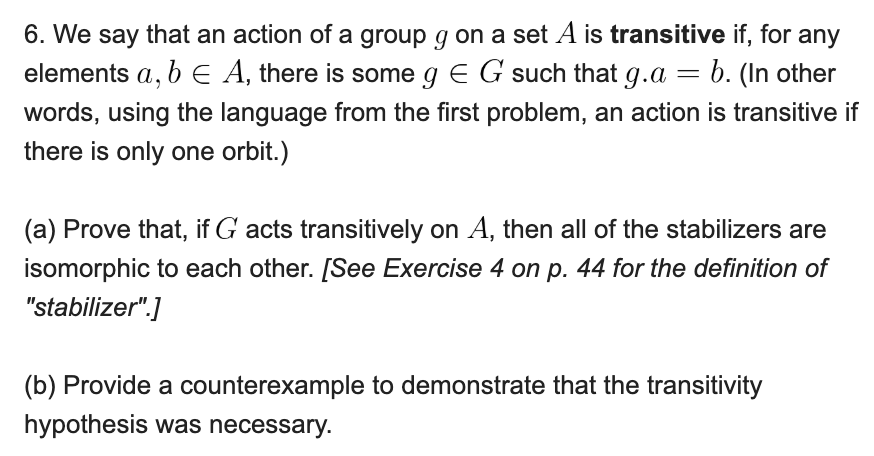
\includegraphics[width=400pt]{img/abstract-algebra--nf--4-50ae.png}
\end{mdframed}

\begin{intuition*}
  \begin{mdframed}
\includegraphics[width=400pt]{img/abstract-algebra--nf--4-a545.png}
\end{mdframed}
\end{intuition*}

{\bf (a)}\\
\begin{proof}
  Let $a, b \in A$ and let $S_a$ and $S_b$ be the stabilizers of $a$ and $b$.

  We wish to show that $S_a \cong S_b$.

  Since $G$ acts transitively on $A$ there exists $g \in G$ such that $ga = b$, and we also
  have $g^{-1}b = a$.

  What might an isomorphism be? We're looking for a map $\varphi$ that sends an element $h \in S_a$ to an
  element $\varphi(h) \in S_b$.

  Well, consider $h \mapsto ghg^{-1}$ (I got this hint from AI). Intuitively, $ghg^{-1}$ is in
  $S_b$ because it corresponds to ``following the $g^{-1}$ edge which takes us from $b$ to $a$, then
  performing $h$, which keeps us at $a$ since $h \in S_a$, then following the $g$ edge which takes us
  back to $b$​''. That intuition corresponds to the
  computation $(ghg^{-1})(b) = g(h(g^{-1}(b))) = g(h(a)) = g(a) = b$.

  Is this a homomorphism? We require $\varphi(hh') = \varphi(h)\varphi(h')$. Yes:
  \begin{align*}
    \varphi(hh')    &= ghh'g^{-1} \\
    \varphi(h)\varphi(h') &= ghg^{-1}gh'g^{-1} = ghh'g^{-1}\\
  \end{align*}

  Is it a bijection? Let's try to find an inverse. Is it $\psi(j) = g^{-1}jg$ for $j \in S_b$? As a
  left-inverse $\psi(\varphi(h)) = \psi(ghg^{-1}) = g^{-1}ghg^{-1}g = h$, and as right
  inverse $\varphi(\psi(j)) = \varphi(g^{-1}jg) = gg^{-1}jgg^{-1} = j$, so yes $\psi$ is an inverse of
  $\varphi$, hence $\varphi$ is a bijective homomorphism, i.e. an isomorphism.

  Since $a, b$ were arbitrary this argument shows that there exists an isomorphism between the
  stabilizers of every pair of elements in $A$.
\end{proof}


{\bf (b)}\\

\begin{proof}
  The above proof relied on the fact that for arbitrary $a, b \in A$ there exists $g \in G$ such
  that $ga = b$, and this fact derived from the hypothesis of transitivity of the action of $G$
  on $A$.

  Let $G$ be the group of rotations of an equilateral triangle, and let $A$ be the set of vertices
  of an equilateral triangle.

  There are two orbits: $\{1, r, r^2\}$ and $\{s, sr, sr^2\}$.






  Suppose we were unable to use that fact. Then there would be an $a, b \in A$ with no edge between
  them in the graph induced by the action of $G$ on $A$.
\end{proof}
